\documentclass[10pt,aspectratio=169]{beamer}
\usepackage{bibentry}
\usepackage[style=bwl-FU]{biblatex}
\usepackage[dvipsnames]{xcolor}
\usepackage{graphicx} % Allows including images
\usepackage{booktabs} % Allows the use of \toprule, 
\usepackage{array}
\usepackage{wrapfig}
\usepackage{graphics}
\usepackage{graphicx}
\usepackage{amsfonts}
\usepackage{amssymb}
\usepackage{amsthm}
\usepackage{textcomp}
% \usepackage{enumitem}
\usepackage{graphicx} % Allows including images
\usepackage{booktabs} % Allows the use of \toprule, 
% \usepackage[nottoc]{tocbibind}
\usepackage{threeparttable}
% \usepackage{natbib}
% \usetheme{SimpleDarkBlue}

\usepackage{mathrsfs}
\usepackage[nospace]{varioref}	
\usepackage{cleveref}

\usepackage{presentation}

\setlength{\parskip}{\baselineskip} 
\graphicspath{{./../Figures}}
% \setlength\itemsep{2em}

\setlength\belowcaptionskip{-3ex}


\usepackage{caption}
\usepackage{subcaption}

\bibliography{../misc/references.bib}



% \institute{NES}

\title{Presentation Title}
% Enter presentation information:
\information%
% Enter link to research paper (optional; comment line if not needed):
[https://github.com/avlsv/CheckingHank]%
% Enter presentation authors:
{Alexander Vlasov (avlasov@nes.ru)}%
% Enter presentation location and date (optional; comment line if not needed):
{New Economic School -- 2024-06-20}

% \usecolortheme{}

% \AtBeginSection{
% 	\begin{frame}
% 		\frametitle{Contents}
% 		\tableofcontents[currentsection]
% 	\end{frame}
% }


\begin{document}

\begin{frame}[fragile, plain]
    \titlepage
\end{frame}



\begin{frame}
    \heading{Research Question}
\end{frame}


\begin{frame}{Systematic Monetary Policy Identification}    
    \begin{block}{Monetary Policy Rule Counterfactuals}
        \begin{itemize}
            \item \cite{McKayWolf2023, BarnichonMesters2023} use the identified shocks and impulse responses to them to minimize a loss function. 
        \end{itemize}
    \end{block}
    \begin{block}{FOMC Preferences}
        \begin{itemize}
            \item  \cite{HIM2023} use \cite{Istrefi2019} data on preferences of FOMC members and using the FOMC rotation mechanism they are able to construct an IV. 
        \end{itemize}
    \end{block}
\end{frame}





\begin{frame}
    \heading{Empirical Approach}
\end{frame}
    


\begin{frame}{State-Dependent LP Model}
    Based on method of \cite{HIM2023}.

    I assume that the monetary policy rule is 
    \[\left(r-r^*\right)_{t+h}=\phi_t^h\mathbb{E}\left[\pi_{t+1}\mid \mathcal{I}_t\right]+\psi_t^h\mathbb{E}\left[x_{t+1}\mid \mathcal{I}_t\right]+\varepsilon_t.\]
    $\mathbb{E}_t\pi_{t+1}$ and $\mathbb{E}_t x_{t+1}$ are the expectations of monetary authority about inflation (deflator/CPI) and output gap (or unemployment gap) at quarter $t+1$.

    Then assuming stimate the following State-Dependent LP-IV.
    \begin{multline*}
        \left(r-r^*\right)_{t+h}=\alpha^h+\beta_\pi^h \hat\pi_t+\gamma_\pi^h \hat\pi_t\left(\mathit{Hawk}_{t}-\overline{\mathit{Hawk}}\right)\\ \beta_u^h \hat x_t+\gamma_u^h \hat u_t\left(\mathit{Hawk}_{t}-\overline{\mathit{Hawk}}\right)\\ +\delta^h\left(\mathit{Hawk}_{t}-\overline{\mathit{Hawk}}\right)+\zeta^hZ+e_{t+h}^h,
    \end{multline*}
\end{frame}


\begin{frame}{HAWK and HAWK IV indexes from \cite{HIM2023}}
    \begin{figure}[h!]
        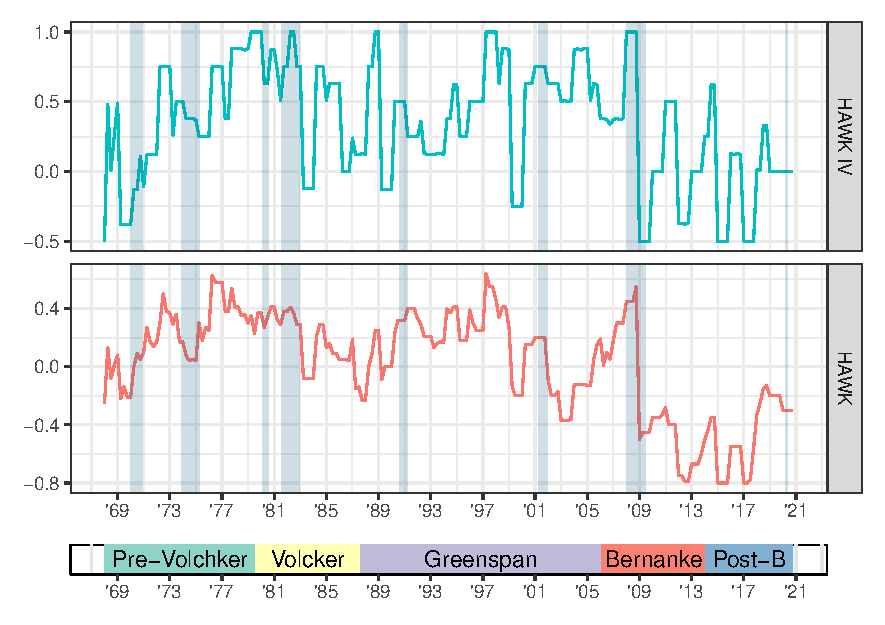
\includegraphics[width=0.7\textwidth]{HAWK_plot_w_heads.pdf}
    \end{figure}
\end{frame}


\begin{frame}{Short and Long Models}
    

\end{frame}










% \begin{frame}{Summary Statistics}
    
% \end{frame}




\section{Results}



\begin{frame}{Short Model. $r-r^*$ Response to Projected CPI Inflation}

    \begin{figure}[!htbp]\centering
        \begin{minipage}{1\textwidth}
            \caption{}
          \begin{subfigure}[b]{0.495\textwidth}
              \centering
              \caption{Average Resp. to Projected CPI Inflation}
              \label{fig:LP_short:average_inflation}
              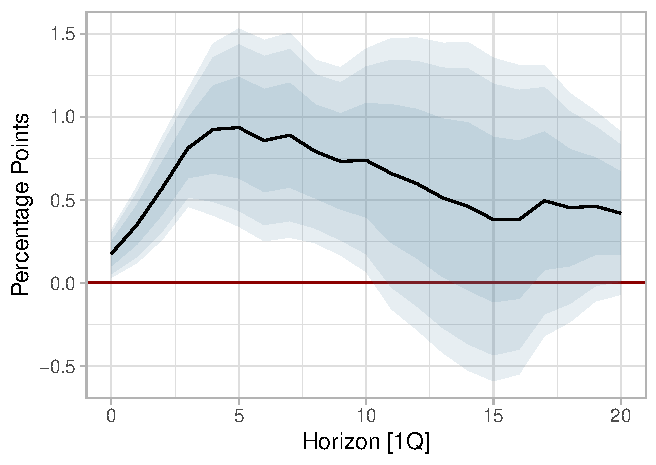
\includegraphics[width=\linewidth]{average_cpi_inflation_short.pdf}
          \end{subfigure}%
          \begin{subfigure}[b]{0.495\textwidth}
              \centering
              \caption{Differential  Resp. to Projected CPI Inflation}
              \label{fig:LP_short:differential_inflation}
              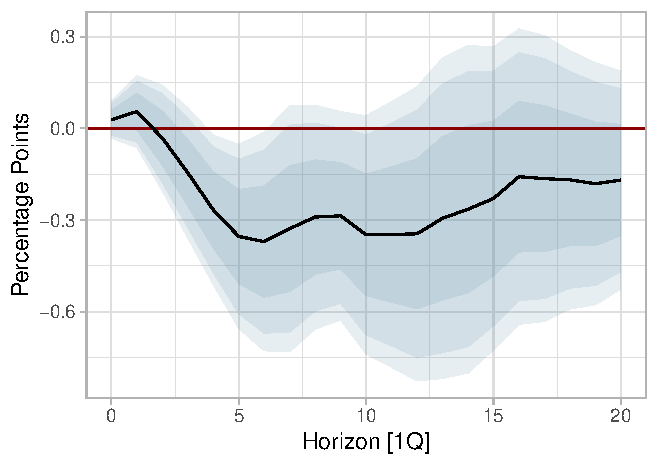
\includegraphics[width=\linewidth]{differential_cpi_inflation_short.pdf}
          \end{subfigure}\vspace{-2ex}
              {\begin{flushleft}\tiny\textit{Notes}: This figure reports the responses of the $(r-r^*)_t$ to an increase in the Tealbook CPI inflation projection and GDP gap projection of 1 p.p. The subfigure \ref{fig:LP_short:average_inflation} reports the response of $(r-r^*)_t$ to projected CPI inflation for the $\mathit{HAWK}$ index equal to the sample average; \ref{fig:LP_short:differential_inflation} is the addition to the response in case there are 2 (out of 12 in total) additional consistent hawks in the FOMC. The shaded areas correspond to 68\%, 90\% and 95\% confidence intervals calculated with \cite{Andrews1991} HAC estimator.\end{flushleft}}
        \end{minipage}
      \end{figure}
\end{frame}

% Subfigures \ref{fig:LP_short:average_gap} and \ref{fig:LP_short:differential_gap} report the same for the increase in projected GDP gap for 1p.p.


\begin{frame}{Short Model. $r-r^*$ Response to Projected GDP Gap}

    \begin{figure}[!htbp]\centering
        \begin{minipage}{1\textwidth}
            \caption{}
          \begin{subfigure}[b]{0.495\textwidth}
              \centering
              \caption{Average Response to Projected GDP Gap}
              \label{fig:LP_short:average_gap}
              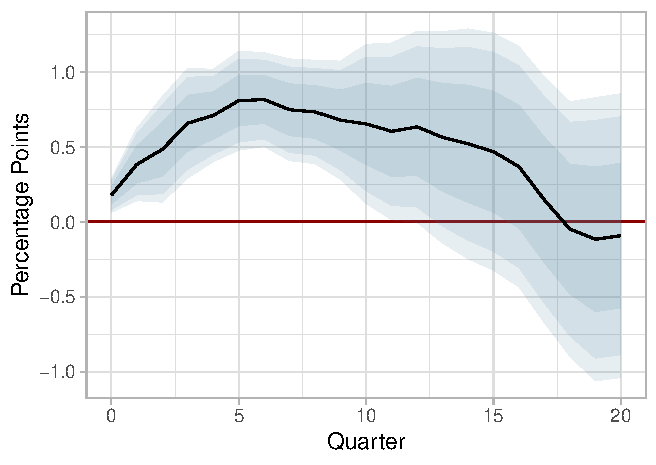
\includegraphics[width=\linewidth]{average_gap_short.pdf}
          \end{subfigure}%
          \begin{subfigure}[b]{0.495\textwidth}
              \centering
              \caption{Differential Response to Projected GDP Gap}
              \label{fig:LP_short:differential_gap}
              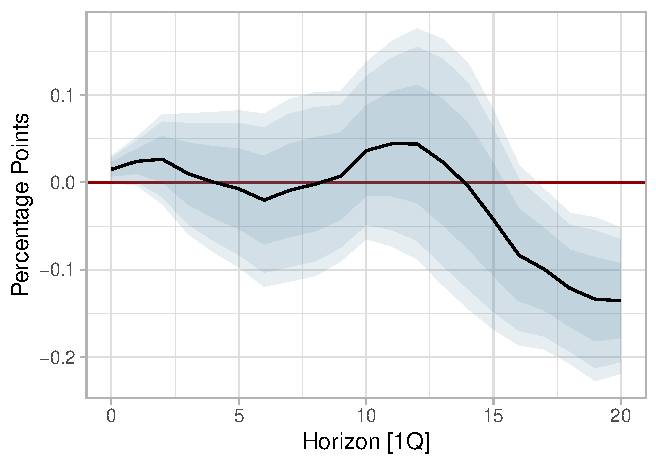
\includegraphics[width=\linewidth]{differential_gap_short.pdf}
          \end{subfigure}
              {\begin{flushleft}\tiny\textit{Notes}: This figure reports the responses of the $(r-r^*)_t$ to an increase in the Tealbook GDP gap projection of 1 p.p. The subfigure \ref{fig:LP_short:average_gap} reports the response of $(r-r^*)_t$ to projected output gap increase for the $\mathit{Hawk}$ index equal to the sample average; \ref{fig:LP_short:differential_gap} is the addition to the previous response in case there are 2 (out of 12 in total) additional consistent hawks in the FOMC. The shaded areas correspond to 68\%, 90\% and 95\% confidence intervals calculated with \cite{Andrews1991} HAC estimator.\end{flushleft}}
        \end{minipage}
      \end{figure}
\end{frame}


\begin{frame}{Long Model. $r-r^*$ Response to Projected Deflator Inflation}

    \begin{figure}[!htbp]\centering
        \caption{}
        \label{fig:LP2}
        \begin{subfigure}[b]{0.48\textwidth}
            \centering
            \caption{Average Response to Inflation}
            \label{fig:average_inflation}
            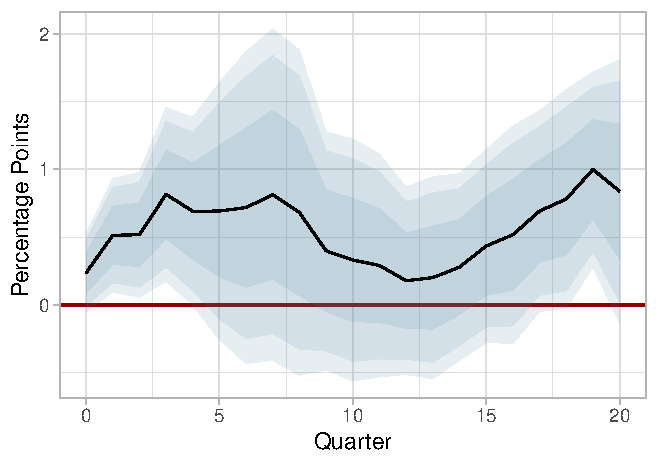
\includegraphics[width=\linewidth]{average_deflator_inflation_long.pdf}
        \end{subfigure}
        \hfill
        \begin{subfigure}[b]{0.48\textwidth}
            \centering 
            \caption{Differential Response to Inflation}
            \label{fig:differential_inflation}
            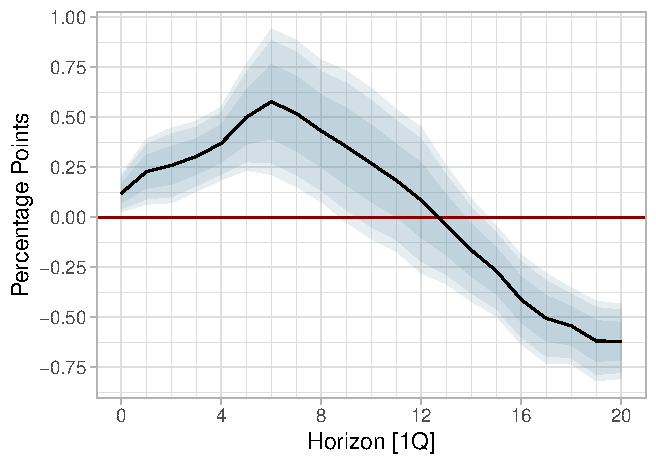
\includegraphics[width=\linewidth]{differential_deflator_inflation_long.pdf}
        \end{subfigure}\vspace{-4ex}
            {\begin{flushleft}\tiny\textit{Notes}: This figure reports the responses of the $(r-r^*)_t$ to an increase in the Tealbook GDP gap projection of 1 p.p. The subfigure \ref{fig:LP_short:average_gap} reports the response of $(r-r^*)_t$ to projected output gap increase for the $\mathit{Hawk}$ index equal to the sample average; \ref{fig:LP_short:differential_gap} is the addition to the previous response in case there are 2 (out of 12 in total) additional consistent hawks in the FOMC. The shaded areas correspond to 68\%, 90\% and 95\% confidence intervals calculated with \cite{Andrews1991} HAC estimator. \end{flushleft}}
    \end{figure}
    
\end{frame}




\begin{frame}{Long Model. $r-r^*$ Response to Projected Unemployment Gap}

    \begin{figure}[!htbp]\centering
    \begin{minipage}{1\textwidth}
        \caption{}
        \label{fig:LP}
        \begin{subfigure}[b]{0.49\textwidth}
            \centering
            \caption{Average Response to Unempl. $\left(\beta_u^h\right)$}
            \label{fig:average_unemployment}
            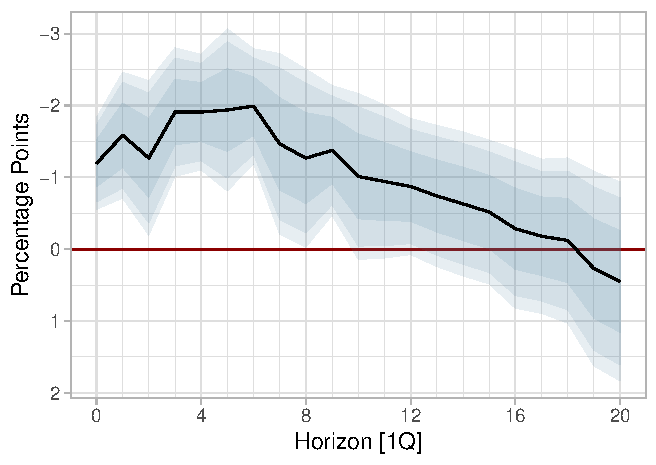
\includegraphics[width=\linewidth]{average_unemployment_long.pdf}
        \end{subfigure}
        \hfill
        \begin{subfigure}[b]{0.49\textwidth}
            \centering
            \caption{Differential Response to Unempl. $\left(\gamma_u^h\right)$}
            \label{fig:differential_unemployment}
            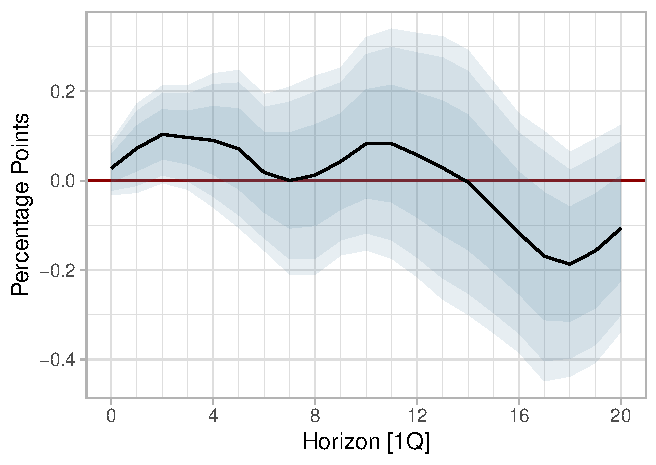
\includegraphics[width=\linewidth]{differential_unemployment_long.pdf}
        \end{subfigure}\vspace{-2ex}
            {\begin{flushleft}\tiny\textit{Notes}: This figure reports the responses of the $(r-r^*)_t$ to an increase in the Tealbook GDP gap projection of 1 p.p. The subfigure \ref{fig:LP_short:average_gap} reports the response of $(r-r^*)_t$ to projected output gap increase for the $\mathit{Hawk}$ index equal to the sample average; \ref{fig:LP_short:differential_gap} is the addition to the previous response in case there are 2 (out of 12 in total) additional consistent hawks in the FOMC. The shaded areas correspond to 68\%, 90\% and 95\% confidence intervals calculated with \cite{Andrews1991} HAC estimator. \end{flushleft}}
        \end{minipage}

    \end{figure}
    
\end{frame}



\begin{frame}
    \heading{Combined IRF}
\end{frame}



\begin{frame}{HAWK and HAWK IV indexes from \cite{HIM2023}}
    \begin{figure}[h!]
        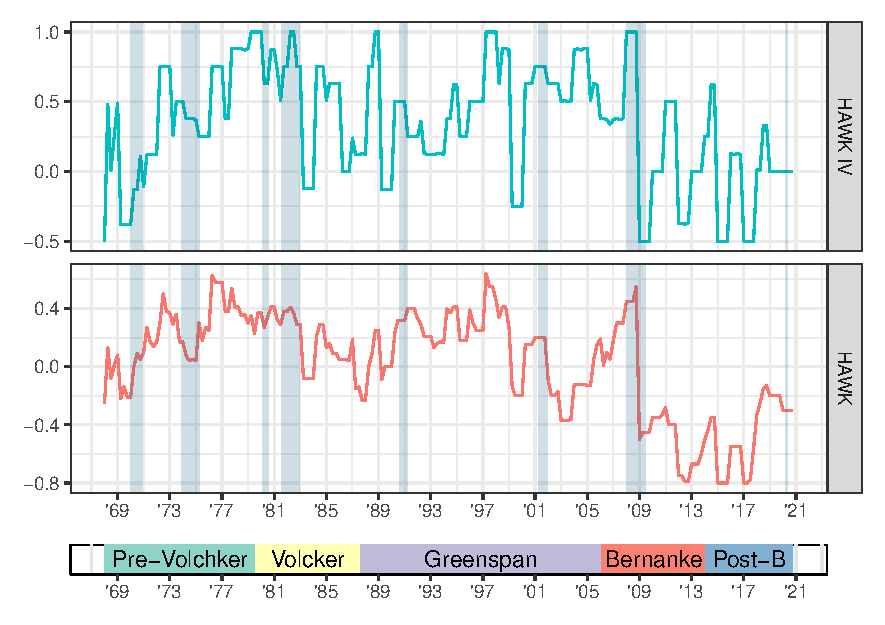
\includegraphics[width=0.7\textwidth]{HAWK_plot_w_heads.pdf}
    \end{figure}
\end{frame}


\begin{frame}{Hawk Index Disected by Fed Chair}
    \begin{figure}
        \begin{minipage}{0.94\textwidth}
            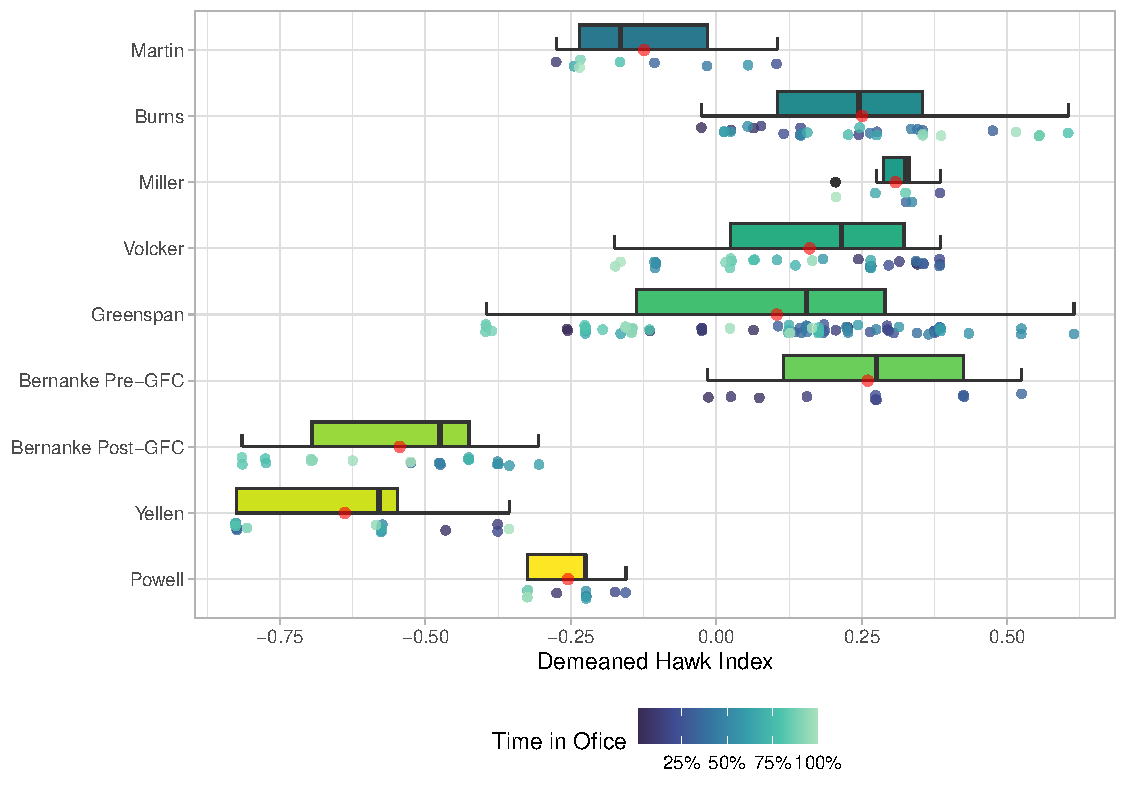
\includegraphics[width=\textwidth]{hawk_by_chair_plot.pdf}
        \end{minipage}
    \end{figure}
\end{frame}



\begin{frame}{Shocks}
    \begin{table}\centering
        \begin{tabular}{rlrrrr}
            \hline
           &  & $\Delta$ CPI inflation & $\Delta$ GDP gap & $\Delta$ Deflator inflation &  $\Delta$ Unemployment gap \\ 
            \hline
          1 & 2008 Q3 & \alr{--2.40} & 0.05 & \alr{--0.05} & 0.49 \\ 
            2 & 2008 Q4 & \alr{--1.45} & \alr{--3.03} & \alr{--0.57} & 1.14 \\ 
            3 & 2009 Q1 & 1.18 & \alr{--2.05} & \alr{--0.40} & 1.36 \\ 
            4 & 2009 Q2 & 1.10 & \alr{--0.21} & 0.03 & 0.87 \\ 
             \hline
          \end{tabular}
    \end{table}
\end{frame} 


\begin{frame}{IRF to}
    \begin{figure}
        \begin{minipage}{.96\textwidth}
            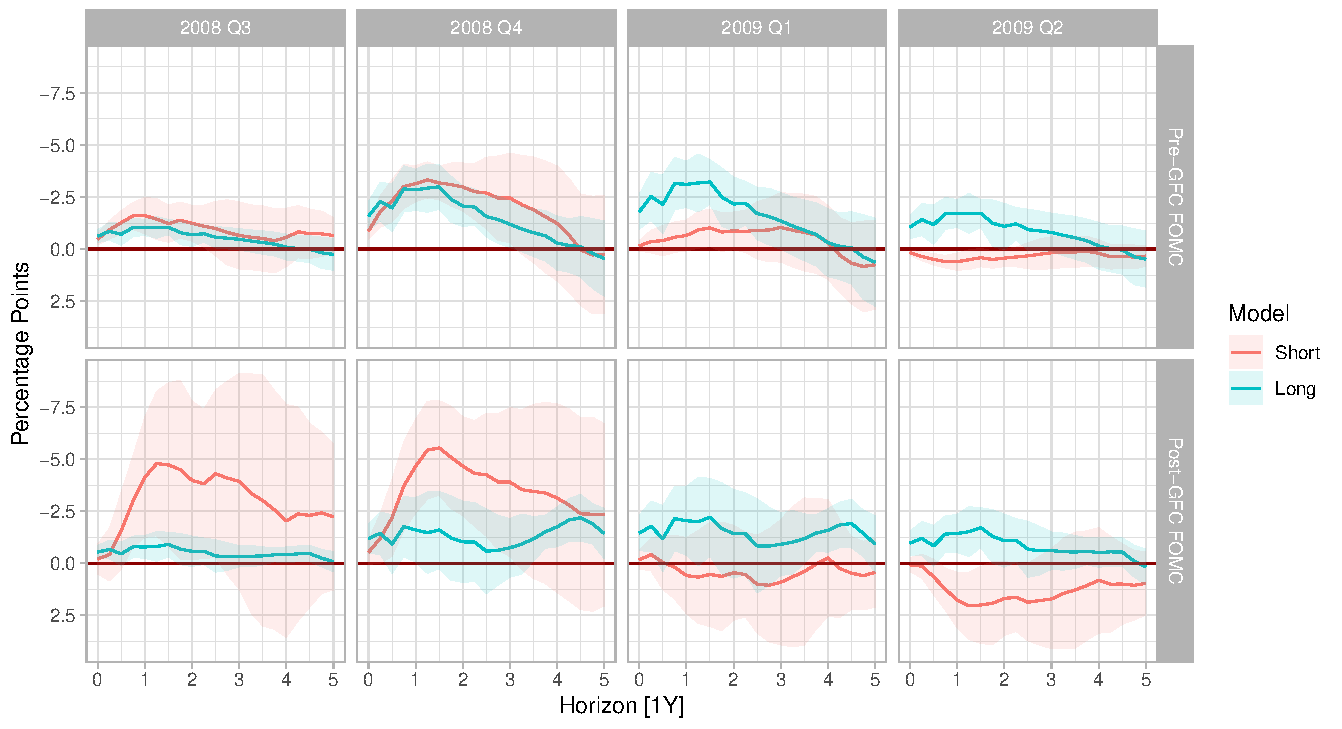
\includegraphics[width=\textwidth]{irfs_combined_gfc_plot.pdf}
        \end{minipage}
    \end{figure}
\end{frame}

\begin{frame}{In-Sample Predictive Ability}
    \begin{figure}
        \begin{minipage}{0.7\textwidth}
            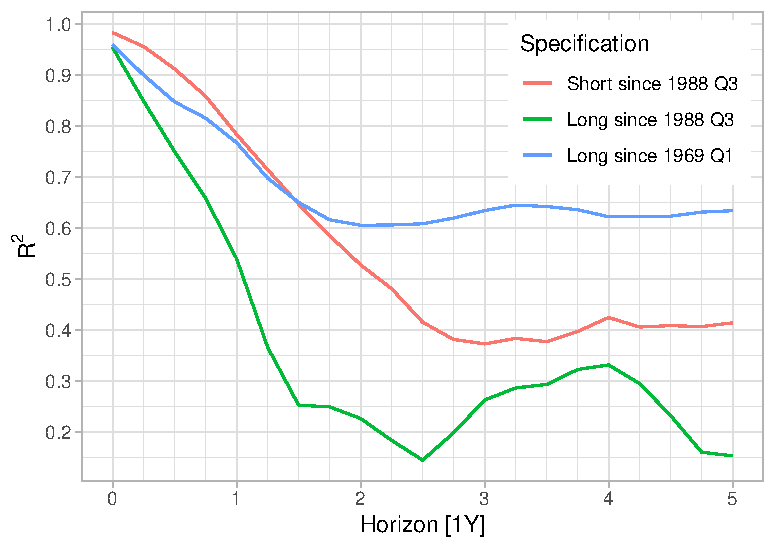
\includegraphics[width=\textwidth]{r_squares_plot.pdf}
        \end{minipage}
    \end{figure}
\end{frame}


\begin{frame}
    \heading{Estimates of Liquidity Premia}
\end{frame}



\begin{frame}{Predicted $r-r^*$ paths}
    \begin{figure}[!htbp]\centering
        \begin{minipage}{\textwidth}
            \caption{}
            \label{fig:predicted_paths}
            \begin{subfigure}[b]{0.49\textwidth}
                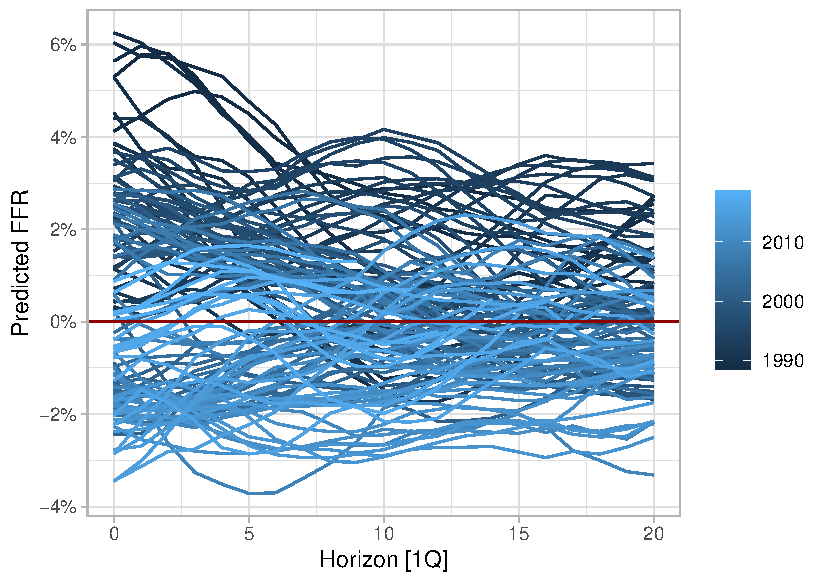
\includegraphics[width=\linewidth]{predicted_paths_short.pdf}
            \end{subfigure}%
            \begin{subfigure}[b]{0.49\textwidth}
          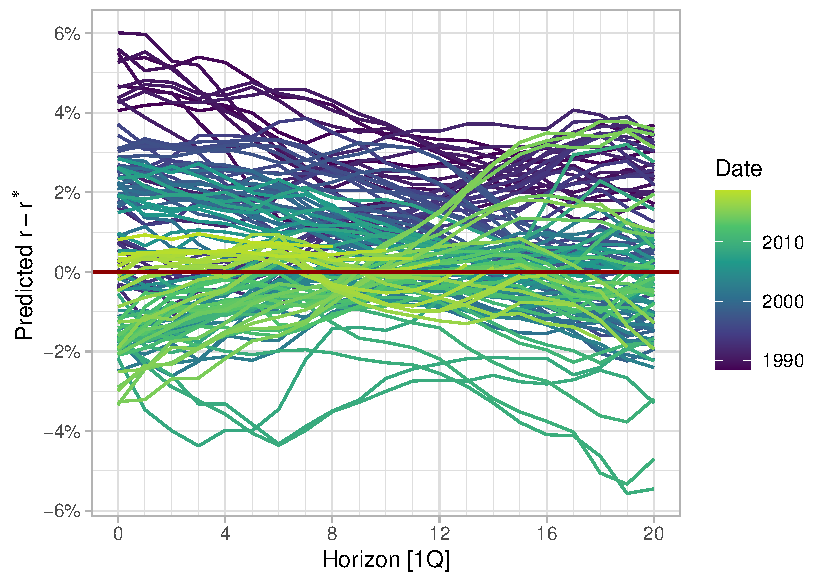
\includegraphics[width=\linewidth]{predicted_paths_long.pdf}
        \end{subfigure}
          {\begin{flushleft}\tiny \textit{Notes:} This figure shows the predictions of $r-r^*$ paths in each state calculated by short and long models.\end{flushleft}} 
          \end{minipage}
      \end{figure}
\end{frame}


\begin{frame}{Predicted FFR paths}
    \begin{figure}[!htbp]\centering
        \begin{minipage}{\textwidth}
            \caption{}
            \label{fig:predicted_paths}
            \begin{subfigure}[b]{0.49\textwidth}
                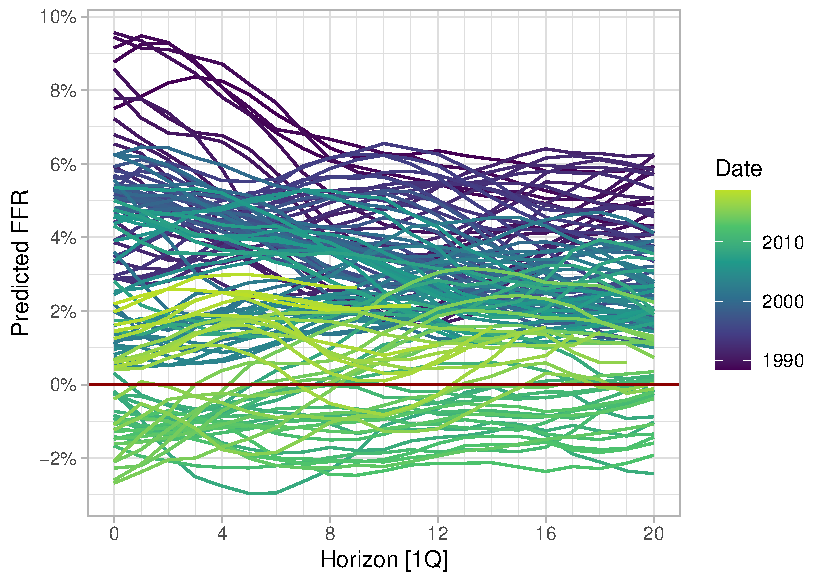
\includegraphics[width=\linewidth]{predicted_ffr_paths_short.pdf}
            \end{subfigure}%
            \begin{subfigure}[b]{0.49\textwidth}
          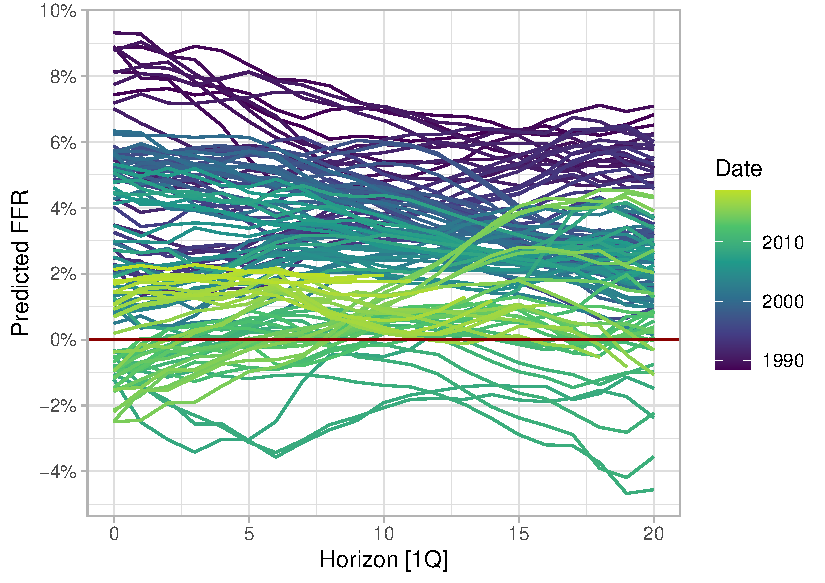
\includegraphics[width=\linewidth]{predicted_ffr_paths_long.pdf}
        \end{subfigure}
          {\begin{flushleft}\tiny \textit{Notes:} This figure shows the predictions of $r$ paths in each state calculated by short and long models.\end{flushleft}} 
          \end{minipage}
      \end{figure}
\end{frame}


\begin{frame}{}
    \begin{figure}\centering 
    \begin{minipage}{0.9\textwidth}\centering
        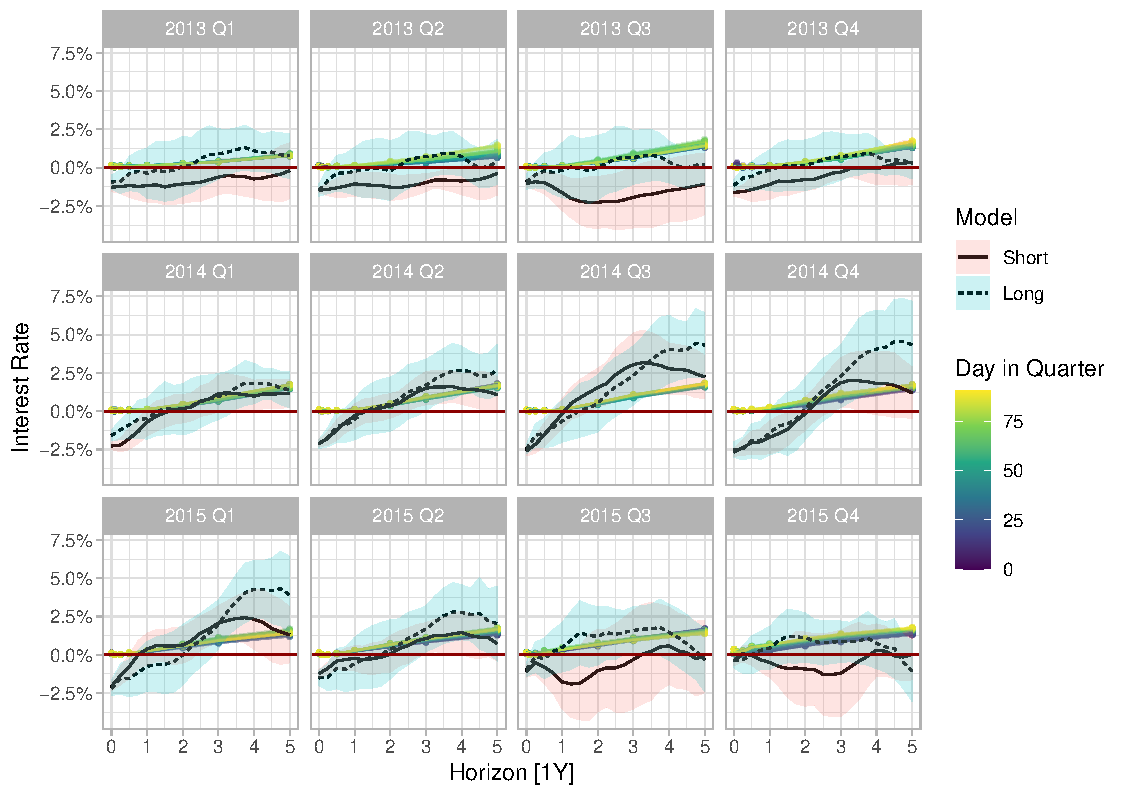
\includegraphics[width=\textwidth]{yield_prediction_plot.pdf}
    \end{minipage}
    \end{figure}
    
\end{frame}


\begin{frame}{Estimates of Liquidity Premia}
    \begin{figure}\centering 
        \begin{minipage}{0.87\textwidth}\centering
        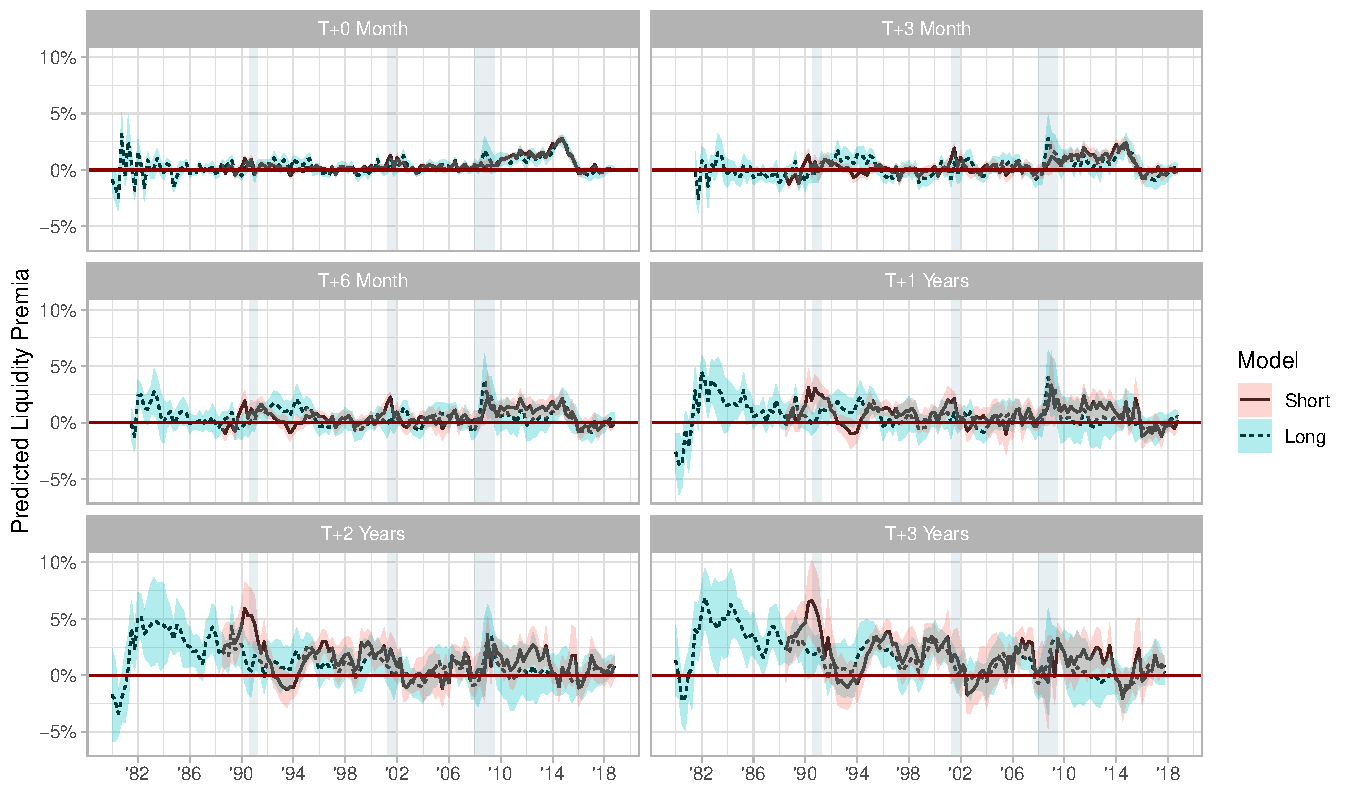
\includegraphics[width=\textwidth]{estimates_of_liquidity_premia_plot.pdf}
        \end{minipage}
    \end{figure}
\end{frame}


\begin{frame}{Estimates of Liquidity Premia Zommed to 2008-2019}
    \begin{figure}\centering 
        \begin{minipage}{0.87\textwidth}\centering
        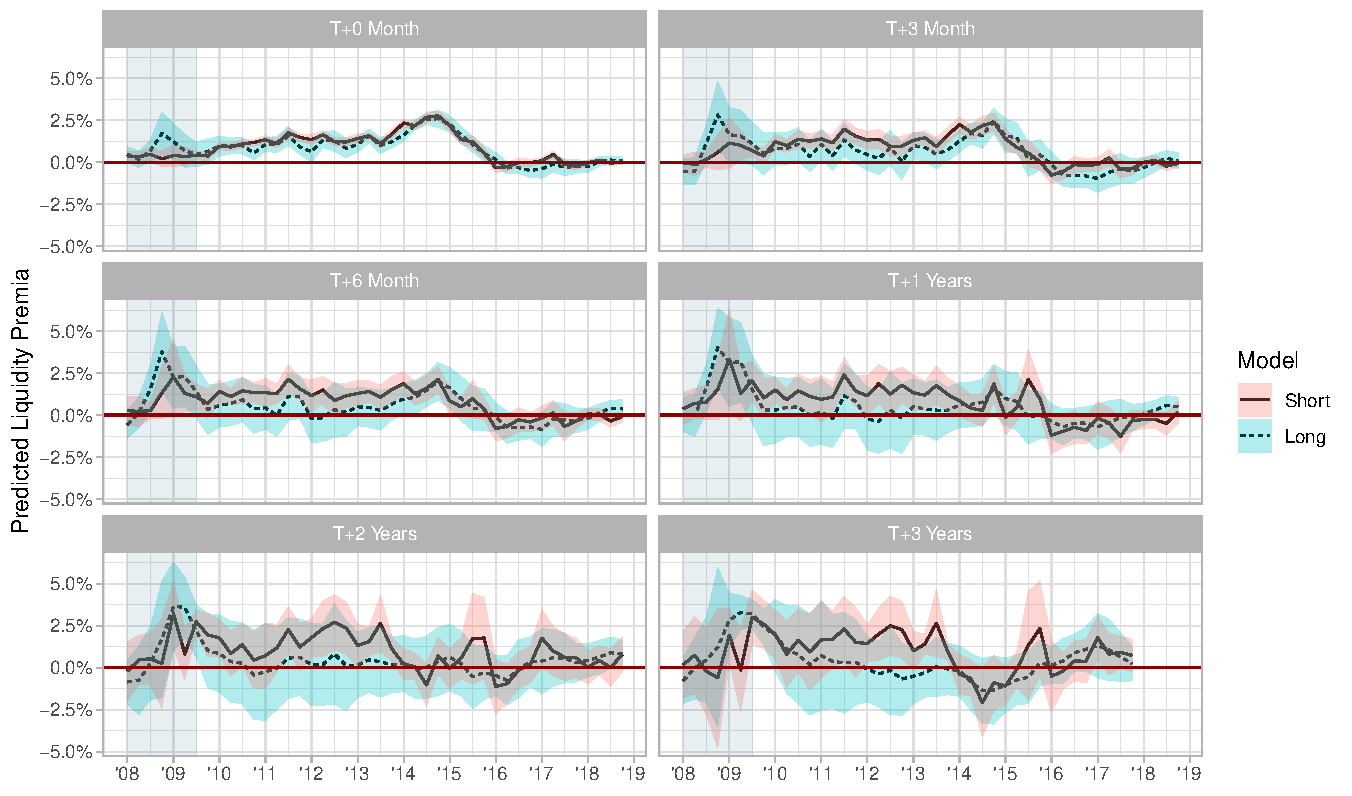
\includegraphics[width=\textwidth]{estimates_of_liquidity_premia_plot_2008.pdf}
        \end{minipage}
    \end{figure}
\end{frame}


\begin{frame}
    \heading{Size-Persistence Estimations}
\end{frame}


\begin{frame}\frametitle{Outcomes of \cite{KMV2018} model}
    \cite{KMV2018} HANK model outcomes:
    \begin{enumerate}
        \item \textbf{\al{Size-Persistence trade-off:}} Cumulative elasticity of aggregate consumption declines with the increase with persistence of monetary policy path in a nonlinear manner.
        \item \textbf{Inflation-Output Tradeoff:} the same Taylor rule shocks lead to the increased effects in Inflation-Output tradeoff.
    \end{enumerate}  
\end{frame}


\begin{frame}{Predicted $r-r^*$ paths}
    \begin{figure}[!htbp]\centering
        \begin{minipage}{\textwidth}
            \caption{}
            \label{fig:predicted_paths}
            \begin{subfigure}[b]{0.49\textwidth}
                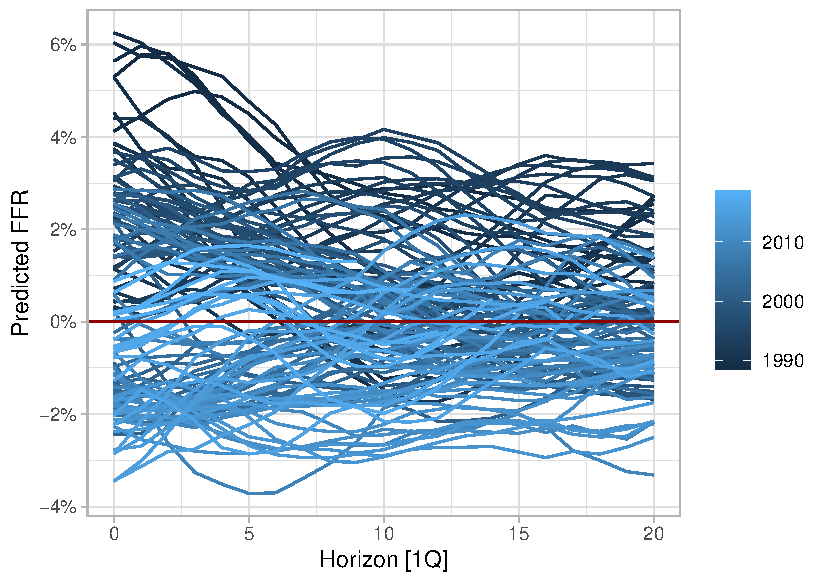
\includegraphics[width=\linewidth]{predicted_paths_short.pdf}
            \end{subfigure}%
            \begin{subfigure}[b]{0.49\textwidth}
          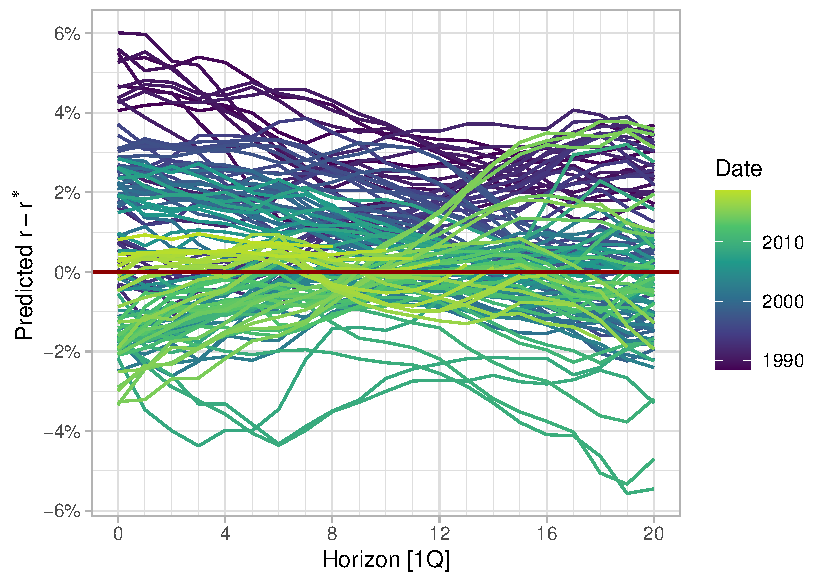
\includegraphics[width=\linewidth]{predicted_paths_long.pdf}
        \end{subfigure}
          {\begin{flushleft}\tiny \textit{Notes:} This figure shows the predictions of $r-r^*$ paths in each state calculated by short and long models.\end{flushleft}} 
          \end{minipage}
      \end{figure}
\end{frame}




\section{Size-Persistence Estimates}

\begin{frame}\frametitle{Size-Persistence in RANK}
    Rate path:
        \begin{equation*}
            r_t=\rho+e^{-\eta t}(r_0-\rho).\label{eq:InterestRatePath}
        \end{equation*}
    
    NK policy    
    \[C_0=\bar C\exp\left(-\frac{1}{\gamma}\int_0^\infty \left(r_s-\rho\right)\,ds\right).\]
    
    Size:
    \begin{equation*}
        R_0=\int_0^\infty \left(r_s-\rho\right)\,ds,\label{eq:KMVsize}
    \end{equation*}
    
    
    \[\frac{-d \log C_0}{dR_0}=\frac{1}{\gamma},\]
    
    
    \end{frame}
    
    % \begin{frame}\frametitle{Picture of Size-Persistence trade-off}
    %     \begin{figure}\centering
    %         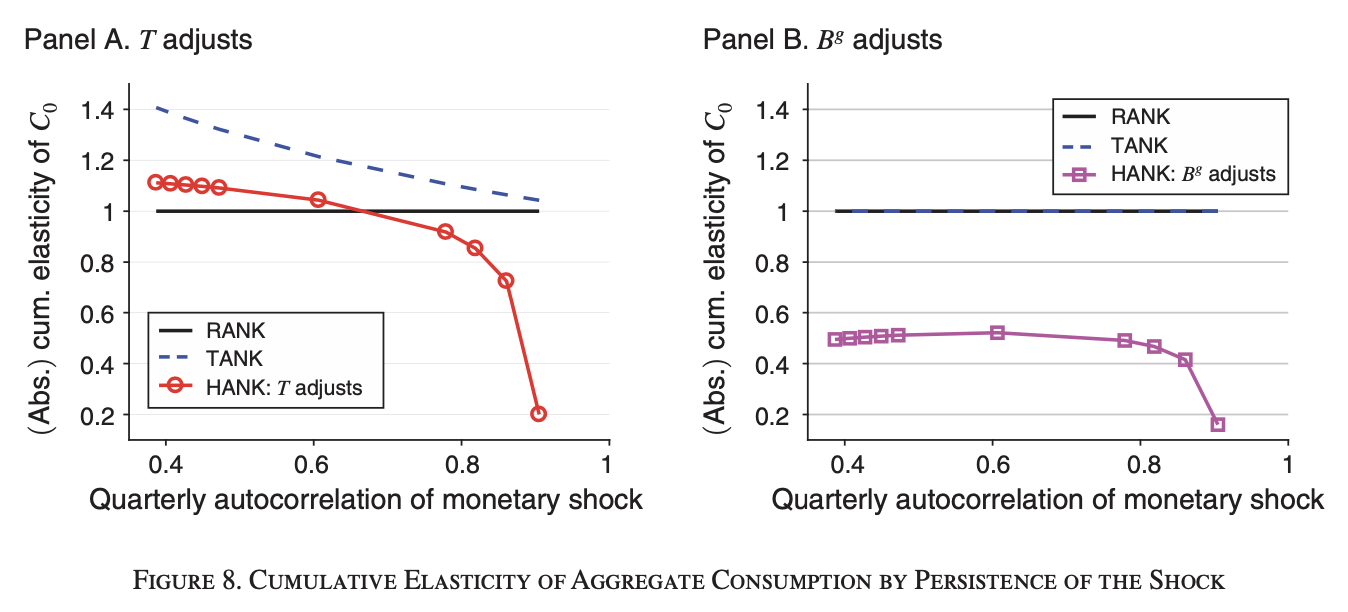
\includegraphics[scale=0.47]{Size_Persistence_KMV.png}
    %         \caption{The difference between the New Keynesian models from \cite{KMV2018}}
    %     \end{figure}
    % \end{frame}
    


    
    % \begin{frame}{Size-Persistent tradeoff by \cite{KMV2018}, formally}
    %     \begin{align}
    %         \textit{RANK:}&\quad& \frac{d}{d\nu}\frac{-d\log C_0}{dR_0}&=0     \label{eq:SizePersistenceRANK}\\
    %     \textit{TANK with $B^g$ adjustment:}&\quad& \frac{d}{d\nu}\frac{-d\log C_0}{dR_0}&= 0     \label{eq:SizePersistenceTANK_B}\\
    %     \textit{TANK with $T$ adjustment:}&\quad& \frac{d}{d\nu}\frac{-d\log C_0}{dR_0}&< 0     \label{eq:SizePersistenceTANK_T}\\
    %     \textit{HANK:}& \quad& 
    %         \frac{d^2}{d\nu ^2}\frac{-d\log C_0}{dR_0}&<0
    %         \label{eq:SizePersistenceHANK}
    %     \end{align}
        
    % \end{frame}

\begin{frame}{Size-Persistence}
    \begin{figure}[!hpbt]\centering
        \begin{minipage}{0.6\textwidth}
          \caption{Estimates of Size and Persistence} 
          \label{fig:size_persistence}
          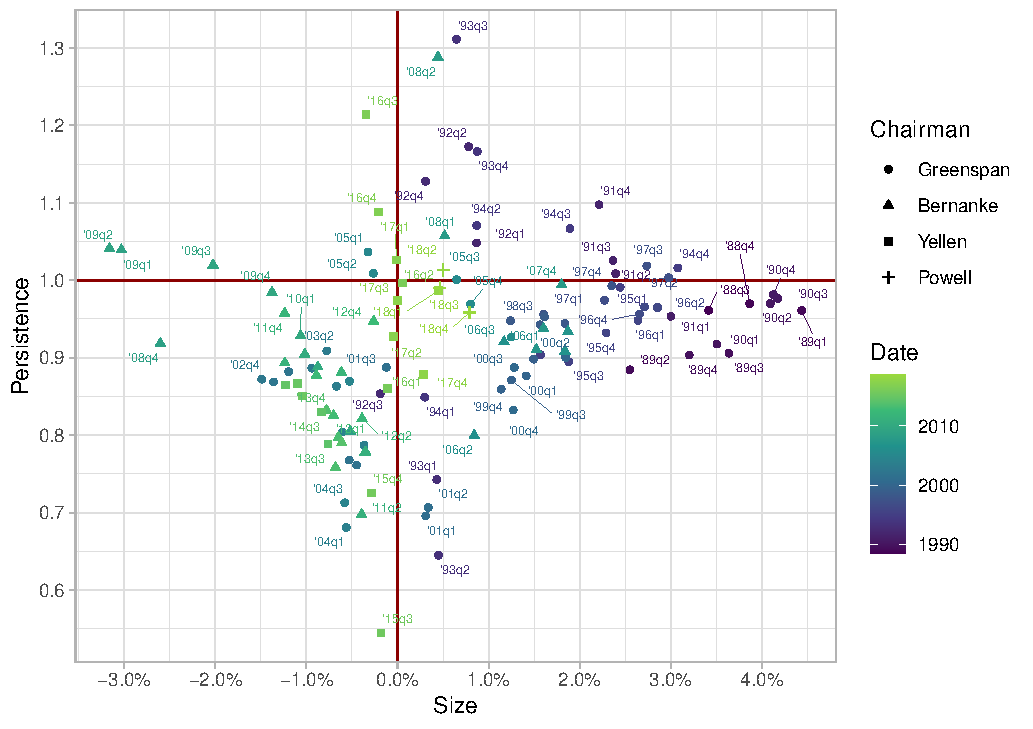
\includegraphics[width=\linewidth]{actual_size_persistence_long.pdf}
        {\begin{flushleft}\tiny \textit{Notes:} \end{flushleft}} 
          \end{minipage}
      \end{figure}
    
\end{frame}


\begin{frame}{Estimates of Size Over Time}
    \begin{figure}[!htbp]\centering
        \caption{}
        \label{fig:Size_Persistence_Dynamics}
        \begin{subfigure}[b]{0.49\textwidth}
            \centering
            \caption{Size Dynamics}
            \label{fig:AverageResponce}
            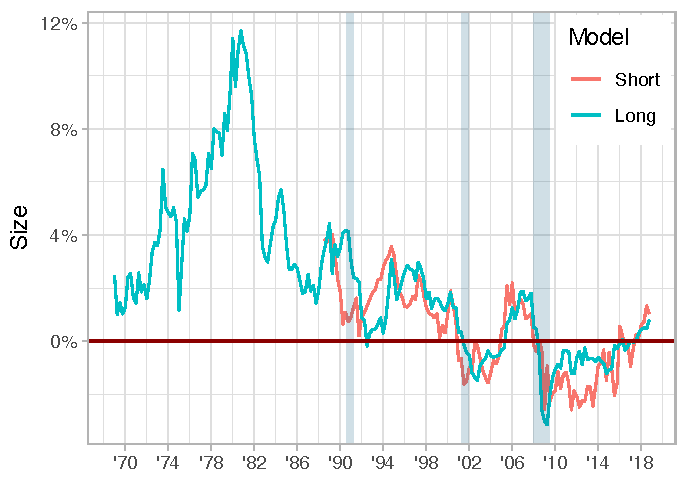
\includegraphics[width=\linewidth]{size_plot.pdf}
        \end{subfigure}%
        \begin{subfigure}[b]{0.49\textwidth}
            \centering
            \caption{Persistence Dynamics}
            \label{fig:DifferentialResponce}
            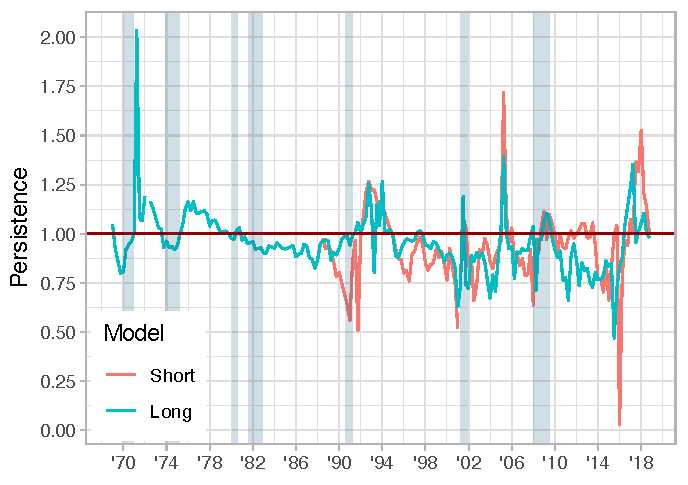
\includegraphics[width=\linewidth]{persistence_plot.pdf}
        \end{subfigure} \vspace{-5ex}
            {\begin{flushleft}\tiny\textit{Notes}: This figure presents the size and persistence, calculated as mean and the first autocorrelation of impulse-response function in each state, constructed as described in \vref{eq:InterestRatePath}, over time. \end{flushleft}}
      \end{figure}
      
\end{frame}







\section{Conclusion}
\begin{frame}\frametitle{Conclusions}
    \begin{block}{So, should we believe in HANK?}
        The evidence above suggests that, we should. 
        At least we have found that consumption behaviour in size-persistent tradeoff corresponds to the TANK model.
    \end{block}
\end{frame}





%Thanks
\lastslide





\appendix
\section{Appendix. Data}

\begin{frame}[label=backupSlide]\frametitle{Data}
    \begin{itemize}\setlength\itemsep{1em}
        \item Projections of FED inflation (deflator, and CPI), GDP gap, unemployment and NAIRU are from Tealbook {\color{gray}
        (average of 1 and 2 quarter quarters ahead following \cite{CoibionGorodnichenko2011} and averaging of FOMC meetings per quarter).}
        \item HAWK index from \cite{HIM2023}.
        \item Natural rate of interest by \cite{HLW2017,HLW2023}.
        \item Short-term rate ($r$) is Fed Funds Rate and \cite{WuXia2016} shadow rate.
        \end{itemize}
    \end{frame}

    \begin{frame}{Rates}
        \begin{figure}[h!]\centering 
            \begin{minipage}{0.7\textwidth}\centering
                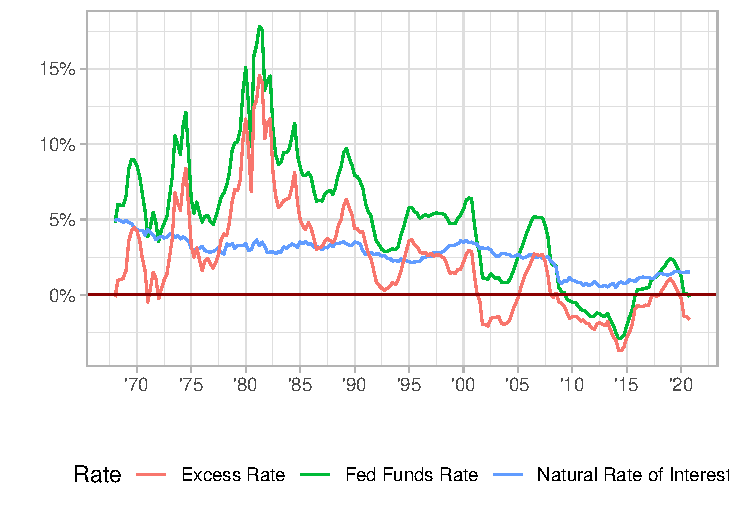
\includegraphics[width=\textwidth]{rate_plot.pdf}
            \end{minipage}
        \end{figure}
    \end{frame}

    \begin{frame}{Tealbook Inflation Projections}
        \begin{figure}[!h]\centering
            \begin{minipage}{0.7\textwidth}\centering
                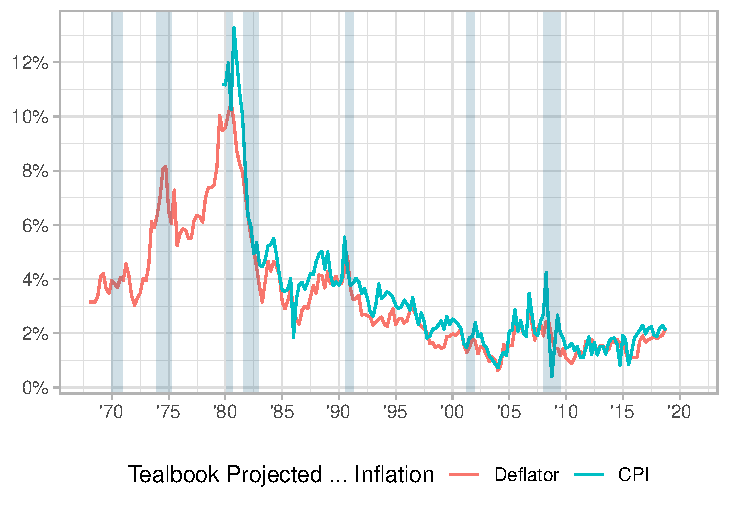
\includegraphics[width=\textwidth]{expected_inflation_plot.pdf}
            \end{minipage}
        \end{figure}
    \end{frame}

    \begin{frame}{Tealbook Unemployment Projections}
        \begin{figure}[!h]\centering
            \begin{minipage}{0.7\textwidth}\centering
                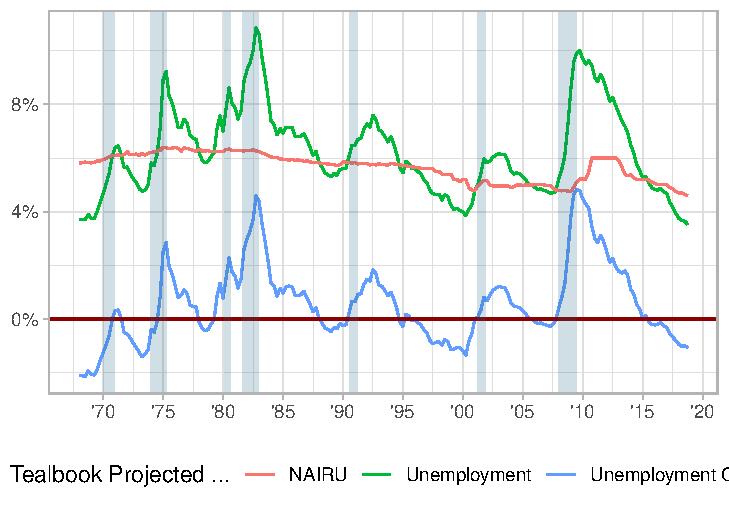
\includegraphics[width=\textwidth]{expected_unemployment_plot.pdf}
            \end{minipage}
        \end{figure}
    \end{frame}



    \begin{frame}{Tealbook Output Gap Projections}
        \begin{figure}[!h]\centering
            \begin{minipage}{0.6\textwidth}\centering
                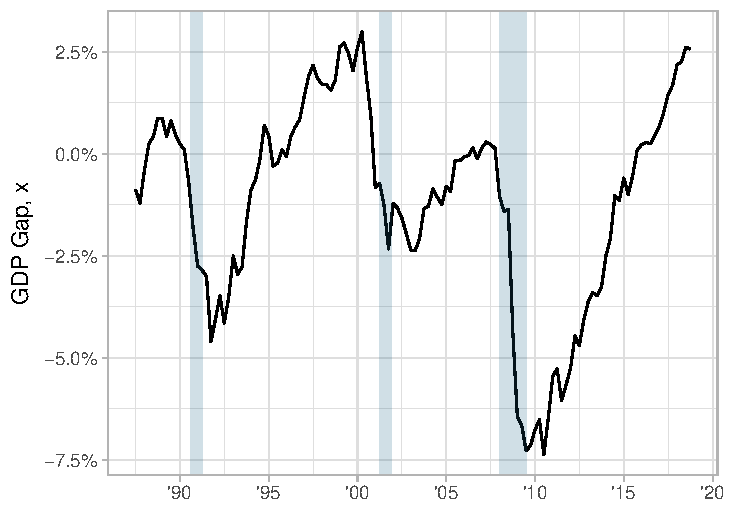
\includegraphics[width=\textwidth]{expected_gap_plot.pdf}
            \end{minipage}
        \end{figure}

    \end{frame}

\begin{frame}[allowframebreaks]{References}
    \footnotesize
    \printbibliography
    \end{frame}
\end{document}